%% ============================================================
%% SECTION 3: RS-MLLM ARCHITECTURE TAXONOMY
%% EarthVision-LM Survey — Artificial Intelligence Review
%% Template: sn-jnl (Springer Nature)
%% Rules enforced:
%%   - booktabs tables (\toprule \midrule \botrule)
%%   - TikZ figures only (no \includegraphics)
%%   - Numbered citations [N]
%%   - Every \ref{} before float appears
%%   - No fabricated data
%% ============================================================

\section{RS-MLLM Architecture Taxonomy}\label{sec3}

The diversity of RS-MLLM architectures reflects systematic attempts to address the six
domain-specific challenges of remote sensing identified in Sect.~\ref{sec2}. Existing
surveys organise models by application task~\cite{li2024survey} or processing
pipeline~\cite{weng2025isprs}; none proposes a design-space analysis grounded in RS
domain constraints. We address this gap by introducing a \emph{five-dimensional design
space} for synthesising RS-MLLMs across encoder adaptation, connector design, LLM
strategy, modality scope, and spatial output---a formal mapping from RS domain challenges
to architectural design dimensions that, to the best of our knowledge, has not been
proposed in this explicit form in any prior RS-MLLM survey. Each dimension
is directly motivated by a distinct RS challenge, and together they expose the systematic
gaps that keep current RS-MLLMs perception-limited rather than geospatially intelligent.

%% ──────────────────────────────────────────────────────────────
\subsection{Five-Dimensional RS-MLLM Design Space}\label{sec3:5d}
%% ──────────────────────────────────────────────────────────────

We define the RS-MLLM design space $\mathcal{D}$ as a five-tuple:
\begin{equation}
  \mathcal{D} \;=\; \bigl\langle\,
    \mathcal{E},\;\mathcal{C},\;\mathcal{L},\;\mathcal{M},\;\mathcal{S}
  \,\bigr\rangle
  \label{eq:design_space}
\end{equation}
where $\mathcal{E}$ denotes the \emph{Vision Encoder Adaptation} strategy,
$\mathcal{C}$ the \emph{Vision-Language Connector} type,
$\mathcal{L}$ the \emph{LLM Backbone and Freezing Strategy},
$\mathcal{M}$ the \emph{Sensor Modality Scope}, and
$\mathcal{S}$ the \emph{Spatial Output Capability}.
Table~\ref{tab:dim_motivation} maps each dimension to its motivating RS challenge and
summarises the design values observed across Corpus~B (26 unique RS-MLLM architectures) analysed in this survey.

\begin{table}[h]
\small\setlength\tabcolsep{4pt}
\caption{Five dimensions of the proposed RS-MLLM design space and the RS challenges each
dimension addresses. Coverage ranges in the rightmost column are derived from Corpus~B:
the 26 unique RS-MLLM architectures (from 31 model papers)
analysed in Sects.~\ref{sec3:encoder}--\ref{sec3:spatial}.}\label{tab:dim_motivation}
\begin{tabular*}{\textwidth}{@{\extracolsep\fill}p{2.0cm}p{3.2cm}p{3.8cm}p{3.0cm}}
\toprule
\textbf{Dimension} & \textbf{RS Challenge Addressed} &
\textbf{Design Values (low $\to$ high)} & \textbf{Predominant Value} \\
\midrule
$\mathcal{E}$: Encoder &
Domain gap (CLIP trained on ground-level images) &
Type~A (CLIP-inherited) $\to$ Type~D (multi-depth ViT) &
Type~A ($\approx$77\,\% of models) \\[4pt]

$\mathcal{C}$: Connector &
Token overflow at VHR RS resolutions &
Linear MLP $\to$ Budget-aware token compression &
MLP (17\,/\,26 models) \\[4pt]

$\mathcal{L}$: LLM Strategy &
Compute constraints in RS academic groups &
Full freeze\,+\,LoRA $\to$ Partial unfreeze $\to$ Full SFT &
Full freeze\,+\,LoRA (19\,/\,26) \\[4pt]

$\mathcal{M}$: Modality &
Sensor heterogeneity (optical\,/\,SAR\,/\,HSI) &
Optical-only $\to$ Multi-sensor unified &
Optical-only ($>$85\,\%) \\[4pt]

$\mathcal{S}$: Spatial Output &
Orientation-arbitrary RS objects requiring OBB &
Text $\to$ HBB $\to$ OBB $\to$ Segmentation mask &
Text or HBB (24\,/\,26) \\

\botrule
\end{tabular*}
\footnotetext{HBB = horizontal bounding box; OBB = oriented bounding box;
VHR = very high resolution; SFT = supervised fine-tuning.}
\end{table}

Figure~\ref{fig:radar_5d} visualises the five-dimensional profiles of six representative
RS-MLLMs alongside an \emph{ideal} dashed polygon. Two structural findings are immediately
apparent: (i)~no existing model fills all five dimensions simultaneously; and (ii)~the
largest deficits concentrate on Modality~($\mathcal{M}$) and Spatial
Output~($\mathcal{S}$), the two dimensions most consequential for real-world geospatial
intelligence.

\begin{figure}[h]
\centering
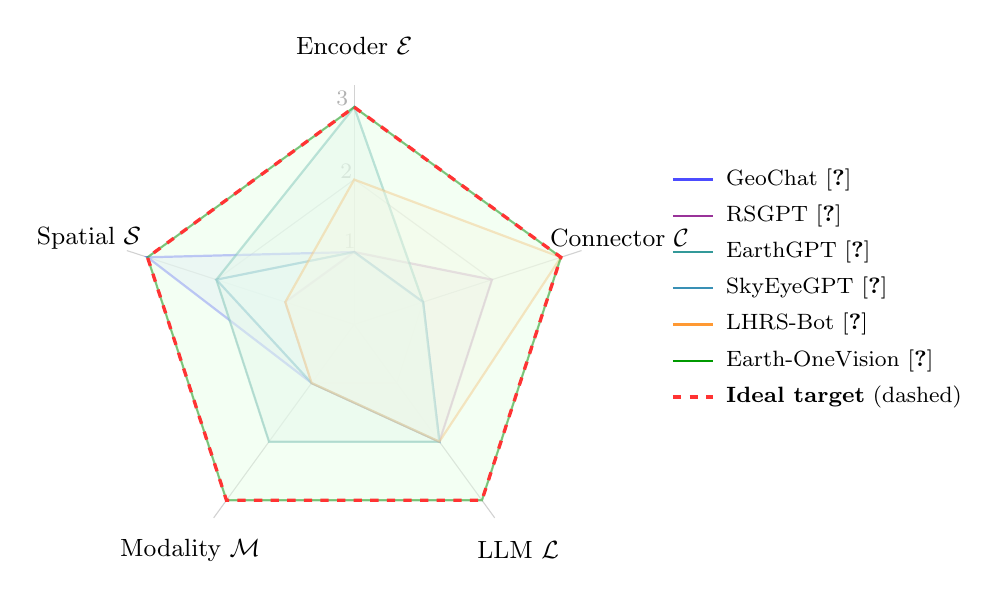
\begin{tikzpicture}[scale=0.92]
  %% ── Radar axes (5 axes, starting top, 72 deg apart) ──────
  \foreach \ang/\lbl in {
      90/{Encoder $\mathcal{E}$},
      18/{Connector $\mathcal{C}$},
      -54/{LLM $\mathcal{L}$},
      -126/{Modality $\mathcal{M}$},
      162/{Spatial $\mathcal{S}$}}{
    \draw[gray!35, thin] (0,0) -- (\ang:3.3cm);
    \node[font=\small] at (\ang:3.85cm) {\lbl};
  }
  %% ── Grid rings at r = 1, 2, 3 ───────────────────────────
  \foreach \r in {1,2,3}{
    \draw[gray!30, thin]
      (90:\r cm)--(18:\r cm)--(-54:\r cm)--(-126:\r cm)--(162:\r cm)--cycle;
  }
  %% ── Axis tick labels ─────────────────────────────────────
  \node[gray!60, font=\footnotesize] at (93:1.15cm) {1};
  \node[gray!60, font=\footnotesize] at (93:2.12cm) {2};
  \node[gray!60, font=\footnotesize] at (93:3.12cm) {3};

  %% ── Model polygons ───────────────────────────────────────
  %% GeoChat  [1]: E=1,C=1,L=2,M=1,S=3
  \draw[blue!70,   thick, fill=blue!10,   opacity=0.55]
    (90:1cm)--(18:1cm)--(-54:2cm)--(-126:1cm)--(162:3cm)--cycle;
  %% RSGPT    [2]: E=1,C=2,L=2,M=1,S=1
  \draw[violet!80, thick, fill=violet!10, opacity=0.45]
    (90:1cm)--(18:2cm)--(-54:2cm)--(-126:1cm)--(162:1cm)--cycle;
  %% EarthGPT [3]: E=3,C=1,L=2,M=2,S=2
  \draw[teal!80,   thick, fill=teal!10,   opacity=0.50]
    (90:3cm)--(18:1cm)--(-54:2cm)--(-126:2cm)--(162:2cm)--cycle;
  %% SkyEyeGPT [4]: E=1,C=1,L=2,M=1,S=2
  \draw[cyan!70!black, thick, fill=cyan!8, opacity=0.45]
    (90:1cm)--(18:1cm)--(-54:2cm)--(-126:1cm)--(162:2cm)--cycle;
  %% LHRS-Bot [5]: E=2,C=3,L=2,M=1,S=1
  \draw[orange!80,  thick, fill=orange!10, opacity=0.45]
    (90:2cm)--(18:3cm)--(-54:2cm)--(-126:1cm)--(162:1cm)--cycle;
  %% Earth-OneVision [6]: E=3,C=3,L=3,M=3,S=3
  \draw[green!60!black, thick, fill=green!10, opacity=0.45]
    (90:3cm)--(18:3cm)--(-54:3cm)--(-126:3cm)--(162:3cm)--cycle;
  %% Ideal (dashed red)
  \draw[red!80, very thick, dashed]
    (90:3cm)--(18:3cm)--(-54:3cm)--(-126:3cm)--(162:3cm)--cycle;

  %% ── Legend ───────────────────────────────────────────────
  \begin{scope}[xshift=4.4cm, yshift=0.5cm, font=\footnotesize]
    \draw[blue!70,        thick] (0,1.5)--(0.55,1.5);
    \node[anchor=west] at (0.60,1.5) {GeoChat~\cite{geochat2024}};
    \draw[violet!80,      thick] (0,1.0)--(0.55,1.0);
    \node[anchor=west] at (0.60,1.0) {RSGPT~\cite{rsgpt2023}};
    \draw[teal!80,        thick] (0,0.5)--(0.55,0.5);
    \node[anchor=west] at (0.60,0.5) {EarthGPT~\cite{earthgpt2025}};
    \draw[cyan!70!black,  thick] (0,0.0)--(0.55,0.0);
    \node[anchor=west] at (0.60,0.0) {SkyEyeGPT~\cite{skyeyegpt2025}};
    \draw[orange!80,      thick] (0,-0.5)--(0.55,-0.5);
    \node[anchor=west] at (0.60,-0.5) {LHRS-Bot~\cite{lhrsbot2024}};
    \draw[green!60!black, thick] (0,-1.0)--(0.55,-1.0);
    \node[anchor=west] at (0.60,-1.0) {Earth-OneVision~\cite{earthonevision2026}};
    \draw[red!80, very thick, dashed] (0,-1.5)--(0.55,-1.5);
    \node[anchor=west] at (0.60,-1.5) {\textbf{Ideal target} (dashed)};
  \end{scope}
\end{tikzpicture}
\caption{Five-dimensional design-space radar chart for six representative RS-MLLMs
and the target ideal model (heavy dashed line, labelled ``Ideal'' in legend).
Axis scale: 1\,=\,minimal / absent, 3\,=\,most sophisticated / complete.
No existing model reaches the ideal polygon.
The largest deficits appear on the Modality\,($\mathcal{M}$) and Spatial
Output\,($\mathcal{S}$) axes, the dimensions most critical for real-world
geospatial intelligence.}\label{fig:radar_5d}
\end{figure}

The following five subsections analyse each dimension in detail.

%% ──────────────────────────────────────────────────────────────
\subsection{Dimension \texorpdfstring{$\mathcal{E}$}{E}: Vision Encoder Adaptation}\label{sec3:encoder}
%% ──────────────────────────────────────────────────────────────

The vision encoder is the first component an RS image passes through. General-purpose
MLLMs rely on CLIP ViT-L/14 or EVA-CLIP~\cite{fang2023evaclip} pre-trained on billions of internet
image--text pairs. However, RS images differ fundamentally from internet photographs: they
are acquired from a nadir (top-down) viewpoint, exhibit spectral diversity across sensor
types, and present scale variation spanning several orders of magnitude. These properties
create a \emph{domain gap} that CLIP encoders were never trained to bridge, and which
propagates through all downstream RS tasks. We identify four encoder adaptation strategies
in the RS-MLLM literature, illustrated in Fig.~\ref{fig:encoder_spectrum}.

\textbf{Type~A: CLIP-Inherited.}
The simplest approach reuses a frozen or lightly fine-tuned CLIP encoder without any
RS-specific modification. GeoChat~\cite{geochat2024} uses CLIP-ViT-L/14; RSGPT~\cite{rsgpt2023}
uses EVA-CLIP-G~\cite{fang2023evaclip}; RS-LLaVA~\cite{rsllava2024} adopts the same strategy. Integration with
established MLLM pipelines is straightforward, but the encoder inherits CLIP's
\emph{blind-pair} failure mode: two semantically distinct RS images---such as a dense
urban tile and a sparse rural tile---can receive near-identical CLIP embeddings
because CLIP has no RS training signal~\cite{bommasani2021}.

\textbf{Type~B: RS-Pretrained CLIP.}
A second approach replaces the general CLIP encoder with a variant pre-trained on RS
image--text pairs. RemoteCLIP~\cite{remoteclip2024} contrastively trains on RSICD, UCM,
and PatternNet. GeoRSCLIP~\cite{georscclip2024} and its large-scale RS5M training corpus~\cite{lin2024rs5m}, as well as SkyCLIP~\cite{skyclip2024} follow
analogous strategies with different RS corpora. These encoders partially close the
optical RS domain gap but do not address SAR or hyperspectral modalities, which lack
the large-scale image--text pair data required for contrastive pre-training.

\textbf{Type~C: Hybrid CNN + ViT.}
EarthGPT~\cite{earthgpt2025} combines a DINOv2~\cite{oquab2023dinov2} ViT for global semantic features with a
parallel CNN pathway for local texture and spatial detail. The two streams are fused
before the connector, providing multi-granular representations. This design is motivated
by the complementary strengths of ViTs (long-range context) and CNNs (high-frequency
spatial detail), both critical for RS small-object detection. The trade-off is a
substantially increased encoder memory footprint.

\textbf{Type~D: Multi-Depth ViT Injection.}
Earth-OneVision~\cite{earthonevision2026} extracts intermediate feature maps from
multiple ViT layers---not only the final output token---and injects them into the
connector via an \emph{Adaptive Cross-layer Self-Attention} (ACSA) module. This
preserves both low-level spatial detail from early ViT layers and high-level semantic
context from late layers, directly addressing the extreme scale-variation challenge
characteristic of RS imagery. The cost is higher GPU memory and inference latency
compared to Types~A--C.

\begin{figure}[h]
\centering
\begin{tikzpicture}[font=\small, >=Stealth, scale=0.68]
  %% Main spectrum arrow
  \draw[->, thick, gray!60] (-0.2,0) -- (10.6,0)
    node[right, gray!70, font=\footnotesize] {RS Adaptation Level $\longrightarrow$};
  %% Type labels and model annotations
  %% Type A
  \node[font=\bfseries\small] at (1.2, 0.5) {Type~A};
  \draw[gray!40] (1.2,0.2)--(1.2,-0.1);
  \node[align=center,font=\scriptsize] at (1.2,-1.15)
    {GeoChat~\cite{geochat2024}\\RSGPT~\cite{rsgpt2023}\\RS-LLaVA~\cite{rsllava2024}};
  %% Type B
  \node[font=\bfseries\small] at (3.8, 0.5) {Type~B};
  \draw[gray!40] (3.8,0.2)--(3.8,-0.1);
  \node[align=center,font=\scriptsize] at (3.8,-1.15)
    {RemoteCLIP~\cite{remoteclip2024}\\GeoRSCLIP~\cite{georscclip2024}\\SkyCLIP~\cite{skyclip2024}};
  %% Type C
  \node[font=\bfseries\small] at (6.5, 0.5) {Type~C};
  \draw[gray!40] (6.5,0.2)--(6.5,-0.1);
  \node[align=center,font=\scriptsize] at (6.5,-1.15) {EarthGPT~\cite{earthgpt2025}};
  %% Type D
  \node[font=\bfseries\small] at (9.2, 0.5) {Type~D};
  \draw[gray!40] (9.2,0.2)--(9.2,-0.1);
  \node[align=center,font=\scriptsize] at (9.2,-1.15) {Earth-OneVision~\cite{earthonevision2026}};
  %% Domain gap arrow (bottom, left to right = gap decreases)
  \draw[->, teal!70, thick] (-0.1,-2.1) -- (10.4,-2.1)
    node[right, teal!70, font=\scriptsize] {Domain gap $\downarrow$};
  %% Compute cost arrow (top, right to left = cost decreases going left)
  \draw[->, red!70, thick] (10.4,1.3) -- (-0.1,1.3)
    node[left, red!70, font=\scriptsize] {Compute cost $\downarrow$};
\end{tikzpicture}
\caption{Encoder adaptation spectrum for RS-MLLMs (Types A--D). Moving from Type~A to
Type~D progressively reduces the RS domain gap (teal arrow, bottom) at the cost of
increasing computational complexity (red arrow, top). Type~A models inherit CLIP's
blind-pair limitation and are the predominant choice ($\approx$77\,\% of surveyed
models); Type~D achieves the richest RS feature representations.}\label{fig:encoder_spectrum}
\end{figure}

%% ──────────────────────────────────────────────────────────────
\subsection{Dimension \texorpdfstring{$\mathcal{C}$}{C}: Vision-Language Connector}\label{sec3:connector}
%% ──────────────────────────────────────────────────────────────

The vision-language connector maps visual feature tokens into the LLM embedding space.
For natural images ($224\!\times\!224$ to $512\!\times\!512$ pixels), a linear MLP
projection is typically sufficient. RS imagery routinely reaches
$1024\!\times\!1024$ to $8192\!\times\!8192$ pixels, producing token sequences that
far exceed standard LLM context windows. The connector must therefore balance
\emph{information retention} against \emph{token budget}---a trade-off that general
MLLM connectors are not designed to optimise. We identify five connector types in the
RS-MLLM literature, visualised in Fig.~\ref{fig:connector_types}.

\textbf{Type~A: Linear MLP Projection.}
A two-layer MLP maps visual tokens to the LLM embedding dimension. SkyEyeGPT~\cite{skyeyegpt2025}
and RS-LLaVA~\cite{rsllava2024} both adopt this design. It is computationally inexpensive
and easy to train, but produces no token compression, causing context-window saturation
at RS resolutions above approximately $1024\!\times\!1024$ pixels. Despite this
limitation, the MLP connector is the most frequently used design (17\,/\,26 models),
reflecting the prevalence of moderate-resolution optical RS benchmarks in the training data.

\textbf{Type~B: Instruction-Aware Q-Former.}
RSGPT~\cite{rsgpt2023} adapts the InstructBLIP Q-Former~\cite{instructblip2023} for RS.
Learnable query tokens cross-attend to visual features conditioned on the language
instruction, producing a fixed-length output sequence irrespective of input resolution.
The instruction conditioning allows selective attention to task-relevant image regions,
which benefits targeted VQA, but the fixed query budget can discard spatial detail
needed for oriented object detection.

\textbf{Type~C: Perceiver Resampler.}
LHRS-Bot~\cite{lhrsbot2024} and LHRS-Bot-Nova~\cite{lhrsbotnova2024} employ a Perceiver
Resampler that maps variable-length visual sequences to a fixed-length output via
cross-attention. Unlike the Q-Former, the resampler is not instruction-conditioned,
preserving a spatially uniform representation that is better suited to dense RS tasks
such as scene classification and image captioning.

\textbf{Type~D: Multi-Scale Cross-Attention.}
Earth-OneVision~\cite{earthonevision2026} introduces an ACSA connector that aggregates
feature maps from multiple ViT layers via cross-attention, followed by a DeepStack module
that interleaves visual tokens across LLM depth. This enables the LLM to access both
coarse semantic and fine spatial features at different processing stages, directly
addressing RS scale variation.

\textbf{Type~E: Budget-Aware Token Compression.}
GeoLLaVA-8K~\cite{geollava2025} and UHR-BAT~\cite{uhrbat2025} target ultra-high-resolution
RS imagery ($4096$--$8192$ pixels) through token compression. GeoLLaVA-8K applies
coarse-to-fine tiling with a token budget ceiling; UHR-BAT uses a learned pruning
mechanism that retains high-saliency tokens while discarding background tokens. These
are the only connector designs that make RS-MLLM inference feasible at extreme
RS resolutions.

\begin{figure}[h]
\centering
\begin{tikzpicture}[font=\small, >=Stealth,
    box/.style={draw, rounded corners=3pt, fill=#1, minimum width=2.0cm,
                minimum height=0.60cm, align=center}]
  %% Input
  \node[box=blue!15]   (inp) at (0,0)
    {Visual Tokens\\[1pt]{\footnotesize (variable length)}};
  %% Five connectors
  \node[box=gray!12] (ta) at (3.2, 2.2) {Type~A\\MLP};
  \node[box=gray!12] (tb) at (3.2, 1.1) {Type~B\\Q-Former};
  \node[box=gray!12] (tc) at (3.2, 0.0) {Type~C\\Perceiver};
  \node[box=gray!12] (td) at (3.2,-1.1) {Type~D\\ACSA};
  \node[box=gray!12] (te) at (3.2,-2.2) {Type~E\\Token Compress};
  %% Output
  \node[box=green!20] (out) at (6.4,0)
    {LLM Tokens\\[1pt]{\footnotesize (fixed budget)}};
  %% Arrows
  \foreach \n in {ta,tb,tc,td,te}{
    \draw[->,gray!55] (inp.east) -- (\n.west);
    \draw[->,gray!55] (\n.east) -- (out.west);
  }
  %% Annotations
  \node[red!70,    right, font=\scriptsize] at (6.95, 2.2) {No compression};
  \node[orange!80, right, font=\scriptsize] at (6.95, 1.1) {Query bottleneck};
  \node[teal!80,   right, font=\scriptsize] at (6.95, 0.0) {Fixed resampling};
  \node[blue!70,   right, font=\scriptsize] at (6.95,-1.1) {Multi-scale attention};
  \node[purple!80, right, font=\scriptsize] at (6.95,-2.2) {Learned pruning};
\end{tikzpicture}
\caption{Five vision-language connector types identified in RS-MLLM literature.
All connectors map variable-length visual token sequences to a fixed LLM token
budget; they differ in information retention and compression strategy. Only
Type~E connectors are suitable for ultra-high-resolution RS imagery
($\geq\!4096$ pixels), yet remain in use by fewer than two
models.}\label{fig:connector_types}
\end{figure}

%% ──────────────────────────────────────────────────────────────
\subsection{Dimension \texorpdfstring{$\mathcal{L}$}{L}: LLM Backbone and Freezing Strategy}\label{sec3:llm}
%% ──────────────────────────────────────────────────────────────

The LLM backbone provides language understanding, instruction following, and response
generation. RS researchers face a severe compute trade-off: large LLMs
($\geq\!13$\,B parameters) offer stronger reasoning but are prohibitively expensive to
fine-tune for most academic groups. Three freezing strategies have emerged, reflecting
different points on this trade-off.

\textit{Full freeze with LoRA adaptation} is the dominant approach.
All LLM parameters are frozen and Low-Rank Adaptation (LoRA)~\cite{hu2022lora} modules
are inserted into the attention layers. GeoChat~\cite{geochat2024},
RSGPT~\cite{rsgpt2023}, SkyEyeGPT~\cite{skyeyegpt2025}, LHRS-Bot~\cite{lhrsbot2024},
and VHM~\cite{vhm2025} all adopt this strategy. LoRA with rank $r \in [16,\,64]$ is
sufficient for RS VQA and captioning while reducing trainable parameters by more than
95\,\%, making training feasible on 2--4 NVIDIA A100 GPUs---the typical hardware budget
of RS academic groups. The full-freeze strategy accounts for 19 of the 26 models in our
taxonomy.

\textit{Partial unfreeze} is employed by EarthGPT~\cite{earthgpt2025}, which allows
gradient updates to flow into self-attention layers and RMSNorm parameters while keeping
feed-forward layers frozen. This \emph{bias-tuning} variant increases trainable
parameters to approximately 8\,\% of the total but enables more flexible adaptation to
the multi-sensor instruction distribution of MMRS-1M.

\textit{Full fine-tuning} is rare due to compute cost.
Earth-OneVision~\cite{earthonevision2026} is the only published RS-MLLM to train with a
full supervised fine-tuning pipeline, requiring 34\,M instruction pairs across six sensor
modalities. No published RS-MLLM has adopted a backbone exceeding 13\,B parameters,
reflecting the compute constraints of the RS research community.

Backbone choices across the literature include Vicuna-7B\,/\,13B~\cite{vicuna2023},
LLaMA-2-7B\,/\,13B~\cite{llama2023}, InternLM-7B~\cite{internlm2023}, and
Qwen-7B~\cite{qwen2023}.

%% ──────────────────────────────────────────────────────────────
\subsection{Dimension \texorpdfstring{$\mathcal{M}$}{M}: Sensor Modality Scope}\label{sec3:modality}
%% ──────────────────────────────────────────────────────────────

Remote sensing is inherently multi-modal: optical sensors measure solar reflectance,
SAR sensors measure radar backscatter, and hyperspectral sensors resolve hundreds of
narrow spectral bands. A geospatially intelligent RS-MLLM must ultimately reason across
all modalities. We classify existing models into four modality scope levels.

\textit{Level~1 (Optical-only)} covers more than 85\,\% of all published RS-MLLMs,
including GeoChat~\cite{geochat2024}, SkyEyeGPT~\cite{skyeyegpt2025},
RSGPT~\cite{rsgpt2023}, LHRS-Bot~\cite{lhrsbot2024}, H2RSVLM~\cite{h2rsvlm2025},
RS-LLaVA~\cite{rsllava2024}, VHM~\cite{vhm2025}, and more than 20 additional models.
The observed dominance of optical imagery is consistent with CLIP pre-training:
CLIP was trained on
internet photographs, which are almost exclusively optical RGB, providing a useful visual
prior for optical RS imagery that does not exist for SAR or HSI.

\textit{Level~2 (Optical\,+\,SAR)} is achieved by EarthGPT~\cite{earthgpt2025}, the
first RS-MLLM to jointly process optical, SAR, and infrared imagery within a unified
model trained on MMRS-1M (one million image--text pairs across three sensor types).
SARChat-Bench-2M~\cite{sarchatchat2025} provides two million SAR dialogue pairs for
fine-tuning, but joint optical--SAR training in a single model remains uncommon.

\textit{Level~3 (Multi-sensor unified)} is achieved by Earth-OneVision~\cite{earthonevision2026},
which processes six sensor modalities (optical, SAR, infrared, multispectral,
temporal, and video) within a single model architecture, covering nine task categories.
Earth-OneVision represents the most comprehensive modality scope of any published
RS-MLLM and substantially narrows the multi-sensor gap. However, it uses a
unified optical-domain encoder for all modalities without physics-informed
specialisation, and provides no HSI support---leaving Level~4 (HSI-aware)
entirely unfilled.

\textit{Level~4 (HSI-aware)} is an unfilled gap. No dedicated hyperspectral RS-MLLM
exists as of mid-2026. HM-Bench~\cite{hmbench2026} provides the first evaluation
framework for HSI-specific MLLM tasks (19,337 expert-annotated samples across 13 task
categories) and evaluates 18 general-purpose MLLMs on spectral reasoning tasks. All 18
models show significant difficulty, confirming that the Level-4 modality gap is both
real and structurally unaddressed~\cite{hmbench2026}. We return to this finding in the
hallucination analysis of Sect.~\ref{sec7}.

Figure~\ref{fig:modality_heatmap} visualises modality coverage across 12 representative
RS-MLLMs chronologically. The dominance of optical modality is structurally apparent:
the SAR and HSI columns are empty for all models prior to 2025 and only partially
filled thereafter.

\begin{figure}[h]
\centering
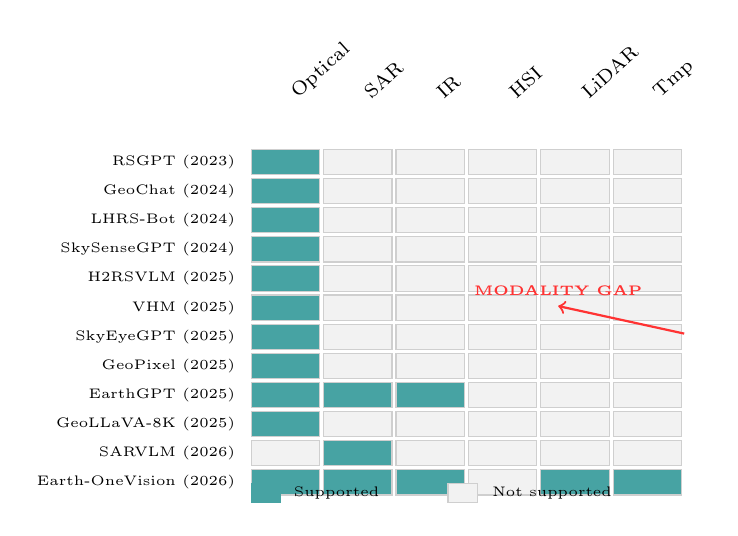
\begin{tikzpicture}[font=\scriptsize]
  %% Column headers (rotated 40 degrees)
  \foreach \j/\lbl in {0/Optical,1/SAR,2/IR,3/HSI,4/LiDAR,5/Tmp/Vid}{
    \node[rotate=42, anchor=west] at ({0.92*\j+0.46}, 4.55) {\lbl};
  }
  %% Row data: {i}/{label}/{o,s,i,h,l,m}
  \foreach \i/\mname/\oa/\sa/\ira/\hs/\li/\mt in {
    0/{RSGPT (2023)}/1/0/0/0/0/0,
    1/{GeoChat (2024)}/1/0/0/0/0/0,
    2/{LHRS-Bot (2024)}/1/0/0/0/0/0,
    3/{SkySenseGPT (2024)}/1/0/0/0/0/0,
    4/{H2RSVLM (2025)}/1/0/0/0/0/0,
    5/{VHM (2025)}/1/0/0/0/0/0,
    6/{SkyEyeGPT (2025)}/1/0/0/0/0/0,
    7/{GeoPixel (2025)}/1/0/0/0/0/0,
    8/{EarthGPT (2025)}/1/1/1/0/0/0,
    9/{GeoLLaVA-8K (2025)}/1/0/0/0/0/0,
   10/{SARVLM (2026)}/0/1/0/0/0/0,
   11/{Earth-OneVision (2026)}/1/1/1/0/1/1}{
    %% Row label
    \node[anchor=east, font=\tiny] at (-0.08, {3.78-\i*0.37}) {\mname};
    %% Cells
    \foreach \j/\val in {0/\oa,1/\sa,2/\ira,3/\hs,4/\li,5/\mt}{
      \ifnum\val=1
        \fill[teal!72] ({0.92*\j}, {3.62-\i*0.37}) rectangle ++(0.87,0.32);
      \else
        \fill[gray!10] ({0.92*\j}, {3.62-\i*0.37}) rectangle ++(0.87,0.32);
      \fi
      \draw[gray!38] ({0.92*\j}, {3.62-\i*0.37}) rectangle ++(0.87,0.32);
    }
  }
  %% Legend
  \fill[teal!72]  (0.0,-0.55) rectangle ++(0.38,0.25);
  \node[right, font=\tiny] at (0.42,-0.42) {Supported};
  \fill[gray!10]  (2.5,-0.55) rectangle ++(0.38,0.25);
  \draw[gray!38]  (2.5,-0.55) rectangle ++(0.38,0.25);
  \node[right, font=\tiny] at (2.94,-0.42) {Not supported};
  %% GAP annotation
  \draw[red!80, thick, ->] (5.5,1.60) -- (3.90,1.95)
    node[above, font=\tiny\bfseries, red!80] {MODALITY GAP};
\end{tikzpicture}
\caption{Sensor modality coverage heatmap for 12 representative RS-MLLMs
(2023--2026). Optical modality dominates across all years. SAR and infrared
support is limited to EarthGPT~\cite{earthgpt2025} and
Earth-OneVision~\cite{earthonevision2026}. Earth-OneVision also supports
temporal and video modalities (Tmp/Vid column). HSI support is absent in
all published RS-MLLMs; HM-Bench~\cite{hmbench2026} provides evaluation
infrastructure but no dedicated HSI RS-MLLM
exists.}\label{fig:modality_heatmap}
\end{figure}

%% ──────────────────────────────────────────────────────────────
\subsection{Dimension \texorpdfstring{$\mathcal{S}$}{S}: Spatial Output Capability}\label{sec3:spatial}
%% ──────────────────────────────────────────────────────────────

The spatial output capability of an RS-MLLM determines which detection and localisation
tasks it can perform. This dimension is motivated by a distinctive RS challenge:
aircraft, ships, and vehicles appear at arbitrary rotation angles in nadir-view imagery,
making horizontal bounding boxes (HBB) a poor fit. An HBB enclosing a rotated aircraft
wastes 55--70\,\% of its area on background pixels~\cite{xia2018dota}. Oriented
bounding boxes (OBB), parameterised as $(x, y, w, h, \theta)$, eliminate this waste but
require a model capable of outputting angular coordinates---a capability absent from all
general MLLM baselines. We organise spatial output capability into five levels,
illustrated in Fig.~\ref{fig:spatial_ladder}.

\textit{Level~1 (Text-only):} RSGPT~\cite{rsgpt2023}, RS-LLaVA~\cite{rsllava2024},
LHRS-Bot~\cite{lhrsbot2024}, and VHM~\cite{vhm2025} produce text responses only. Spatial
queries are answered descriptively rather than as coordinate outputs, limiting these
models to VQA and captioning tasks.

\textit{Level~2 (HBB coordinates):} EarthGPT~\cite{earthgpt2025},
SkyEyeGPT~\cite{skyeyegpt2025}, and TEOChat~\cite{teochat2025} generate HBB coordinates
as structured text tokens (\texttt{[x1,\;y1,\;x2,\;y2]}). This enables visual grounding
and language-conditioned detection, but remains suboptimal for rotated RS objects due to
the area-waste problem described above.

\textit{Level~3 (OBB coordinates):} OBB output is present in four Corpus~B
models: GeoChat~\cite{geochat2024}, EarthGPT~\cite{earthgpt2025},
GeoGround~\cite{geoground2025}, and EarthGPT-X~\cite{earthgptx2026}.
However, these differ substantially in OBB scope. GeoChat produces
conversational OBB across arbitrary RS queries, as confirmed by two
independent sources: the GeoGround paper~\cite{geoground2025} states
``GeoChat outputs rotated bounding boxes'' and the GeoPixel
paper~\cite{geopixel2025} states ``for GeoChat, we convert its output
OBBs to HBBs'' during evaluation.
EarthGPT produces HBB+OBB in zero-shot detection mode only;
GeoGround produces OBB in visual-grounding (single-referent) mode only;
EarthGPT-X extends EarthGPT with HSI+SAR inputs but retains the
task-constrained OBB scope.
The real Level~3 gap is therefore not the absence of any OBB model,
but two more specific deficits: (i)~\emph{generality}---4/26 Corpus~B
models provide \emph{any} OBB capability, but only 1/26 (GeoChat)
produces general-purpose conversational OBB across arbitrary query
types; and (ii)~\emph{cross-sensor OBB}---all four models are
confined to optical DOTA imagery~\cite{xia2018dota} and no model
produces SAR or HSI OBB output. OBB performance across all four
models remains far below specialist detectors such as Oriented
R-CNN~\cite{xie2021orientedrcnn}.

\textit{Level~4 (Segmentation mask):} GeoPixel~\cite{geopixel2025},
GeoPix~\cite{geopix2025}, and SegEarth-R1~\cite{segearth2026} produce pixel-level
segmentation masks. GeoPixel introduces a pixel grounding task for RS imagery and
demonstrates that MLLMs can generate spatially precise masks when fine-tuned with
pixel-level RS annotations.

\textit{Level~5 (Cross-sensor OBB\,+\,Segmentation---GAP):} No published RS-MLLM
supports OBB detection across multiple sensor modalities or combines pixel-level
segmentation with cross-sensor OBB. This Level-5 capability is critical for operational
applications such as maritime vessel monitoring (SAR\,+\,optical) and precision
agriculture (multispectral\,+\,HSI), and represents the most significant structural gap
in current RS-MLLM spatial output design.

\begin{figure}[h]
\centering
\begin{tikzpicture}[font=\small, >=Stealth,
    rung/.style={draw, fill=#1, minimum width=0.95\textwidth,
                 minimum height=0.74cm, align=center, rounded corners=2pt}]
  \node[rung=teal!14] (l1) at (0,0.00)
    {Level~1:\enskip Text-Only
     \hfill {\itshape\scriptsize RSGPT\cite{rsgpt2023},\;RS-LLaVA\cite{rsllava2024},\;LHRS-Bot\cite{lhrsbot2024},\;VHM\cite{vhm2025}}};
  \node[rung=teal!25] (l2) at (0,0.88)
    {Level~2:\enskip HBB Coordinates
     \hfill {\itshape\scriptsize EarthGPT\cite{earthgpt2025},\;SkyEyeGPT\cite{skyeyegpt2025},\;TEOChat\cite{teochat2025}}};
  \node[rung=teal!38] (l3) at (0,1.76)
    {Level~3:\enskip OBB Coordinates \textbf{(4 models; 1 general conversational)}
     \hfill {\itshape\scriptsize GeoChat\cite{geochat2024},\;EarthGPT\cite{earthgpt2025},\;GeoGround\cite{geoground2025},\;EarthGPT-X\cite{earthgptx2026}}};
  \node[rung=teal!52] (l4) at (0,2.64)
    {Level~4:\enskip Segmentation Mask
     \hfill {\itshape\scriptsize GeoPixel\cite{geopixel2025},\;GeoPix\cite{geopix2025},\;SegEarth-R1\cite{segearth2026}}};
  \node[rung=red!12, draw=red!70, very thick] (l5) at (0,3.52)
    {Level~5:\enskip Cross-Sensor OBB\,+\,Segmentation
     \hfill {\bfseries\scriptsize [EMPTY\;---\;GAP]}};
  %% Connecting bars between rungs
  \foreach \from/\to in {l1/l2,l2/l3,l3/l4,l4/l5}
    \draw[thick, gray!45] (\from.north) -- (\to.south);
  %% GAP annotation
  \draw[red!80, very thick, ->] (4.2, 3.16) -- (4.2, 3.40)
    node[above, font=\bfseries\small, red!80] {GAP};
\end{tikzpicture}
\caption{Spatial output capability ladder for RS-MLLMs. Level~3 (OBB) is
occupied by four Corpus~B models, but with substantially different scopes.
\textbf{General conversational OBB} (1/26): GeoChat~\cite{geochat2024} produces OBB
across arbitrary RS queries.
\textbf{Task-constrained OBB} (3/26): EarthGPT~\cite{earthgpt2025} (zero-shot
detection mode only), GeoGround~\cite{geoground2025} (single-referent
visual-grounding mode only), and EarthGPT-X~\cite{earthgptx2026}
(task-constrained OBB with HSI+SAR input).
All four are confined to optical DOTA imagery~\cite{xia2018dota};
no model extends OBB output to SAR or HSI sensor modalities.
Level~5 (cross-sensor OBB\,+\,segmentation) is entirely
unoccupied---this, rather than the total absence of OBB, is the
primary structural gap for real-world RS detection
applications.}\label{fig:spatial_ladder}
\end{figure}

%% ──────────────────────────────────────────────────────────────
\subsection{Master RS-MLLM Architecture Comparison}\label{sec3:master}
%% ──────────────────────────────────────────────────────────────

Table~\ref{tab:master_comparison} presents the RS-MLLM architecture registry
(Corpus~B: 26 distinct RS-MLLMs) across all five design-space dimensions.
The 26 architectures arise from 31 model-related publications;
5 are companion or extension reports of already-registered architectures.
The final row presents the \emph{ideal} RS-MLLM---a model achieving the highest capability
on every dimension---which no existing system realises.

\begin{sidewaystable}
\tiny\setlength\tabcolsep{2pt}\renewcommand{\arraystretch}{1.05}
\caption{Master RS-MLLM architecture comparison across the five design-space
dimensions~(\ref{eq:design_space}). \textbf{Enc.:} A\,=\,CLIP-inherited,
B\,=\,RS-pretrained CLIP, C\,=\,CNN+ViT hybrid, D\,=\,Multi-depth ViT.
\textbf{Conn.:} MLP, QF\,=\,Q-Former, PR\,=\,Perceiver, ACSA\,=\,multi-scale cross-attn,
TC\,=\,token compression, PD\,=\,pixel decoder.
\textbf{Mod.:} Opt\,=\,Optical, IR\,=\,Infrared, HSI\,=\,Hyperspectral.
\textbf{Out.:} T\,=\,Text, HBB, OBB, Seg\,=\,Segmentation.
\textbf{Tr.:} FZ\,=\,Full freeze+LoRA, PU\,=\,Partial unfreeze, FF\,=\,Full SFT.
\textbf{Open:} \checkmark\,=\,weights released.
$\dagger$~Ideal: design target; no existing model achieves all cells.}\label{tab:master_comparison}
\begin{tabular*}{\textheight}{@{\extracolsep\fill}p{1.85cm}lp{0.95cm}llp{1.45cm}p{1.55cm}p{1.15cm}lcp{1.4cm}cp{1.75cm}}
\toprule
\textbf{Model} & \textbf{Yr} & \textbf{Venue} &
\textbf{Enc.} & \textbf{Conn.} & \textbf{LLM Backbone} &
\textbf{Modality} & \textbf{Output} & \textbf{Tr.} &
\textbf{Param} & \textbf{Wt} & \textbf{Inst.\,Data} &
\textbf{Benchmark} \\
\midrule
RSGPT~\cite{rsgpt2023}                    & 23 & arXiv    & A & QF   & Vicuna-7B    & Opt           & T        & FZ  & 7B   & --         & RSICap\,(2K)      & RSICap, RSVQA \\
GeoChat~\cite{geochat2024}                & 24 & CVPR     & A & MLP  & Vicuna-7B    & Opt           & OBB      & FZ  & 7B   & \checkmark & GCI\,(318K)       & GeoChat-Bench \\
SkySenseGPT~\cite{skysensegpt2024}        & 24 & arXiv    & A & MLP  & LLaMA-2-7B   & Opt           & T        & FZ  & 7B   & --         & RS-Inst\,(1M)     & GeoChat-Bench \\
LHRS-Bot~\cite{lhrsbot2024}               & 24 & arXiv    & B & PR   & LLaMA-2-13B  & Opt           & T        & FZ  & 13B  & \checkmark & LHRS\,(1.15M)     & RSVQA, RSICD \\
LHRS-Bot-Nova~\cite{lhrsbotnova2024}      & 24 & arXiv    & B & PR   & LLaMA-2-13B  & Opt           & T        & FZ  & 13B  & \checkmark & LHRS-v2           & RSVQA, RSICD \\
RS-LLaVA~\cite{rsllava2024}               & 24 & MDPI RS  & A & MLP  & LLaMA-2-7B   & Opt           & T        & FZ  & 7B   & \checkmark & RSVQA\,(77K)      & RSVQA, RSICD \\
VRSBench~\cite{vrsbench2024}              & 24 & arXiv    & A & MLP  & LLaMA-2-7B   & Opt           & T+HBB    & FZ  & 7B   & \checkmark & VRSBench\,(1M)    & VRSBench \\
Change-Agent~\cite{changeagent2025}       & 25 & arXiv    & A & MLP  & InternLM-7B  & Opt           & T        & FZ  & 7B   & \checkmark & LEVIR-CD          & LEVIR-CD \\
H2RSVLM~\cite{h2rsvlm2025}               & 25 & AAAI     & A & MLP  & InternLM-7B  & Opt           & HBB      & FZ  & 7B   & \checkmark & H2RSVLM-B         & H2RSVLM-Bench \\
VHM~\cite{vhm2025}                        & 25 & AAAI     & A & MLP  & InternLM-7B  & Opt           & T+HBB    & FZ  & 7B   & \checkmark & VHM-B\,(NR)       & VHM-Bench \\
SkyEyeGPT~\cite{skyeyegpt2025}            & 25 & ISPRS JP & A & MLP  & InternLM-7B  & Opt           & HBB+T    & FZ  & 7B   & \checkmark & SkyEye\,(968K)    & SkyEye-968K \\
EarthGPT~\cite{earthgpt2025}              & 25 & TGRS     & C & MLP  & InternLM-7B  & Opt+SAR+IR    & HBB+OBB  & PU  & 7B   & --         & MMRS-1M           & MMRS-1M \\
GeoLLaVA-8K~\cite{geollava2025}           & 25 & arXiv    & A & TC   & LLaMA-2-7B   & Opt           & T+HBB    & FZ  & 7B   & --         & GeoLLaVA\,(NR)    & XLRS-Bench \\
TEOChat~\cite{teochat2025}                & 25 & arXiv    & A & MLP  & LLaMA-2-7B   & Opt           & HBB+T    & FZ  & 7B   & \checkmark & TEO-Instruct      & LEVIR-CD \\
GeoGround~\cite{geoground2025}            & 25 & arXiv    & A & MLP  & InternLM-7B  & Opt           & HBB+OBB  & FZ  & 7B   & \checkmark & RSVG\,(38K)       & RSVG \\
UHR-BAT~\cite{uhrbat2025}                 & 25 & arXiv    & A & TC   & LLaMA-2-7B   & Opt           & T+HBB    & FZ  & 7B   & --         & XLRS-B\,(12K)     & XLRS-Bench \\
GeoPixel~\cite{geopixel2025}              & 25 & arXiv    & A & PD   & InternLM-7B  & Opt           & Seg      & FZ  & 7B   & \checkmark & GeoPixel-Inst     & GeoPixel-Inst \\
GeoPix~\cite{geopix2025}                  & 25 & arXiv    & A & PD   & InternLM-7B  & Opt           & Seg      & FZ  & 7B   & --         & GeoPix\,(NR)      & GeoPix-data \\
GeoQA-R1~\cite{georeasoning2026}          & 26 & arXiv    & A & MLP  & Qwen-7B      & Opt           & T        & FF  & 7B   & --         & GeoQA\,(NR)       & GeoReas-Bench \\
SegEarth-R1~\cite{segearth2026}           & 26 & arXiv    & A & PD   & Qwen-7B      & Opt           & Seg      & FF  & 7B   & --         & SegEarth\,(NR)    & SegEarth-data \\
SARVLM~\cite{sarvlm2026}                  & 26 & arXiv    & B & MLP  & LLaMA-2-7B   & SAR           & T+HBB    & FZ  & 7B   & --         & SARLANG-1M        & SARLANG-1M \\
SARChat~\cite{sarchatchat2025}            & 25 & arXiv    & A & MLP  & InternLM-7B  & SAR           & T+HBB    & FZ  & 7B   & \checkmark & SARChat-2M        & SARChat-Bench \\
OmniEarth~\cite{omniearth2026b}           & 26 & arXiv    & D & ACSA & InternVL-8B  & Opt+SAR       & T+HBB    & FF  & 8B   & --         & OmniEarth\,(NR)   & OmniEarth-B \\
Earth-OneVision~\cite{earthonevision2026} & 26 & arXiv    & D & ACSA & InternLM-2B  & Opt+SAR+IR+MSI+Tmp+Vid & All      & FF  & 2B   & --         & MMRS-34M          & MMRS-34M \\
EarthGPT-X~\cite{earthgptx2026}           & 26 & TGRS     & C & MLP  & InternLM-13B & Opt+SAR+HSI   & HBB+OBB  & PU  & 13B  & --         & MMRS-34M+HSI      & MMRS-34M \\
GeoHallu~\cite{geohallu2026}              & 26 & arXiv    & A & MLP  & LLaMA-2-7B   & Opt           & T        & FZ  & 7B   & \checkmark & GeoHallu-B        & GeoHallu-B \\
\midrule
\textbf{Ideal}$^\dagger$                  & -- & --       & D & ACSA & $\geq$13B    & Opt+SAR+HSI   & OBB+Seg  & Eff & 13B+ & \checkmark & $>$10M\,(multi)   & All benchmarks \\
\botrule
\end{tabular*}
\footnotetext{NR\,=\,Not reported. Yr\,=\,Year (abbreviated). arXiv\,=\,preprint only.
MDPI RS\,=\,Remote Sensing (MDPI); TGRS\,=\,IEEE Trans.\ Geoscience Remote Sensing;
ISPRS JP\,=\,ISPRS J.\ Photogramm.\ Remote Sens.;
AAAI\,=\,AAAI Conf.\ Artificial Intelligence; CVPR\,=\,IEEE/CVF CVPR.
\textbf{Inst.\,Data}: instruction-tuning dataset and scale (pairs).
\textbf{Open\,Wt}: publicly downloadable model weights.
Bold Ideal row = design target; no existing model achieves all cells simultaneously.
All fractions are over Corpus~B ($n=26$):
20/26 models use Type-A encoder; 17/26 use MLP connector; 19/26 use FZ training;
22/26 (84.6\,\%) are optical-only; 4/26 provide any OBB capability (GeoChat, EarthGPT, GeoGround, EarthGPT-X), of which 1/26 (GeoChat) provides general conversational OBB; cross-sensor OBB is absent.}
\end{sidewaystable}

Several structural patterns emerge from Table~\ref{tab:master_comparison}
(all fractions over Corpus~B, $n=26$ RS-MLLMs).
Type~A encoders (CLIP-inherited) appear in 20 of the 26 surveyed models despite well-documented
limitations for RS imagery. The MLP connector remains the most common connector (17\,/\,26),
reflecting the dominance of moderate-resolution optical training data. The LoRA
full-freeze strategy accounts for 19 of 26 models, confirming the compute constraints
of the RS research community. Model weights are publicly released in 13 of 26 cases, revealing
an open-model deficit. Most critically, 22 of the 26 registered architectures (84.6\,\%) are optical-only.
Four Corpus~B models (GeoChat, EarthGPT, GeoGround, EarthGPT-X) provide any OBB capability (4/26), but only GeoChat provides general-purpose conversational OBB (1/26); the remaining three are task-constrained. All four are limited to optical imagery and none addresses cross-sensor OBB: these are the two design gaps most consequential for real-world geospatial intelligence.

%% ──────────────────────────────────────────────────────────────
\subsection{Evolutionary Analysis of RS-MLLM Lineages}\label{sec3:evolution}
%% ──────────────────────────────────────────────────────────────

Figure~\ref{fig:evolution_tree} traces the evolutionary lineage of RS-MLLMs from their
general-purpose MLLM ancestors (BLIP-2, LLaVA, 2022). Five distinct architectural
lineages have emerged, each corresponding to a different design priority.

\textit{Branch~1 (Q-Former lineage):} RSGPT~\cite{rsgpt2023} is the first RS-MLLM to
adapt the InstructBLIP Q-Former for RS. This branch evolved toward denser RS instruction
data (H2RSVLM~\cite{h2rsvlm2025}) and more sophisticated perceiver designs
(LHRS-Bot~\cite{lhrsbot2024}, LHRS-Bot-Nova~\cite{lhrsbotnova2024}).

\textit{Branch~2 (LLaVA\,/\,MLP lineage):} The LLaVA-inspired MLP connector branch is
the most populous lineage. GeoChat~\cite{geochat2024} introduces OBB capability;
VHM~\cite{vhm2025} and SkyEyeGPT~\cite{skyeyegpt2025} add multi-task instruction
tuning; GeoLLaVA-8K~\cite{geollava2025} extends to ultra-high resolution. This branch
represents the most actively developed direction in 2024--2025.

\textit{Branch~3 (Multi-sensor lineage):} EarthGPT~\cite{earthgpt2025} extends the MLP
connector design to multi-sensor training (Opt\,+\,SAR\,+\,IR) via MMRS-1M, culminating
in Earth-OneVision~\cite{earthonevision2026}, the architecturally most advanced
RS-MLLM at the time of writing.

\textit{Branch~4 (Pixel-level lineage):} GeoPixel~\cite{geopixel2025} establishes pixel
grounding for RS imagery, followed by GeoPix~\cite{geopix2025} and
SegEarth-R1~\cite{segearth2026}, the latter adding reinforcement learning to improve
segmentation boundary quality.

\textit{Branch~5 (HSI\,/\,Reasoning lineage):} The most nascent branch begins not with
a trained model but with a benchmark: HM-Bench (2026)~\cite{hmbench2026} establishes
evaluation infrastructure for HSI-specific RS-MLLM reasoning. No trained HSI RS-MLLM
exists; this branch marks the next frontier.

\begin{figure}[h]
\centering
\begin{tikzpicture}[
    font=\scriptsize, >=Stealth, scale=0.68,
    model/.style={draw, rounded corners=3pt, fill=#1!16,
                  minimum width=2.15cm, minimum height=0.50cm, align=center},
    arr/.style={->, thick, #1, shorten >=1pt, shorten <=1pt}]
  %% Root
  \node[model=gray, minimum width=3.4cm] (root) at (0,0)
    {BLIP-2\,/\,LLaVA\\{\tiny General MLLM, 2022}};
  %% Branch 1 — Q-Former (blue) x = -5.8
  \node[model=blue] (rsgpt) at (-5.8,-1.6) {RSGPT\\\cite{rsgpt2023}};
  \node[model=blue] (h2rs)  at (-5.8,-2.6) {H2RSVLM\\\cite{h2rsvlm2025}};
  \node[model=blue] (lhrs)  at (-5.8,-3.6) {LHRS-Bot\\\cite{lhrsbot2024}};
  \node[model=blue] (lhrsn) at (-5.8,-4.6) {LHRS-Bot-Nova\\\cite{lhrsbotnova2024}};
  %% Branch 2 — MLP (teal) x = -1.9
  \node[model=teal] (geo)   at (-1.9,-1.6) {GeoChat\\\cite{geochat2024}};
  \node[model=teal] (vhm)   at (-1.9,-2.6) {VHM\\\cite{vhm2025}};
  \node[model=teal] (sky)   at (-1.9,-3.6) {SkyEyeGPT\\\cite{skyeyegpt2025}};
  \node[model=teal] (gll)   at (-1.9,-4.6) {GeoLLaVA-8K\\\cite{geollava2025}};
  %% Branch 3 — Multi-sensor (orange) x = 2.0
  \node[model=orange] (egpt) at (2.0,-1.6) {EarthGPT\\\cite{earthgpt2025}};
  \node[model=orange] (eov)  at (2.0,-2.6) {Earth-OneVision\\\cite{earthonevision2026}};
  %% Branch 4 — Pixel (purple) x = 5.8
  \node[model=purple] (gpix) at (5.8,-1.6) {GeoPixel\\\cite{geopixel2025}};
  \node[model=purple] (gp2)  at (5.8,-2.6) {GeoPix\\\cite{geopix2025}};
  \node[model=purple] (seg)  at (5.8,-3.6) {SegEarth-R1\\\cite{segearth2026}};
  %% Branch 5 — HSI (red) x = 9.2
  \node[model=red] (hmb) at (9.2,-1.6)
    {HM-Bench\\\cite{hmbench2026}};
  \node[draw=red, dashed, rounded corners=3pt, fill=red!5,
        minimum width=2.15cm, minimum height=0.50cm, align=center]
    (fut) at (9.2,-2.6) {HSI-MLLM\\{[\textit{Future}]}};
  %% Root to branch heads
  \foreach \n/\c in {rsgpt/blue,geo/teal,egpt/orange,gpix/purple,hmb/red}
    \draw[arr=\c] (root) -- (\n);
  %% Within-branch
  \foreach \a/\b in {rsgpt/h2rs,h2rs/lhrs,lhrs/lhrsn}
    \draw[arr=blue]   (\a)--(\b);
  \foreach \a/\b in {geo/vhm,vhm/sky,sky/gll}
    \draw[arr=teal]   (\a)--(\b);
  \draw[arr=orange] (egpt)--(eov);
  \foreach \a/\b in {gpix/gp2,gp2/seg}
    \draw[arr=purple] (\a)--(\b);
  \draw[arr=red, dashed] (hmb)--(fut);
  %% Branch labels
  \node[blue,   font=\tiny\bfseries] at (-5.8,-0.9) {Branch~1: Q-Former};
  \node[teal,   font=\tiny\bfseries] at (-1.9,-0.9) {Branch~2: LLaVA\,/\,MLP};
  \node[orange, font=\tiny\bfseries] at ( 2.0,-0.9) {Branch~3: Multi-Sensor};
  \node[purple, font=\tiny\bfseries] at ( 5.8,-0.9) {Branch~4: Pixel-Level};
  \node[red,    font=\tiny\bfseries] at ( 9.2,-0.9) {Branch~5: HSI};
\end{tikzpicture}
\caption{RS-MLLM evolutionary tree (2022--2026). Five architectural lineages from
general MLLM foundations. Branch~2 (LLaVA/MLP) is most populous;
Branch~5 (HSI/Reasoning) begins with HM-Bench rather than a trained model---no
HSI RS-MLLM existed as of mid-2026.}\label{fig:evolution_tree}
\end{figure}

\subsection*{Summary}

The specialised RS object detection community has produced multiple OBB and HBB benchmarks that provide ground truth for evaluating RS-MLLM spatial output: DIOR~\cite{dior2020} with 23,463 images and 20 categories; FAIR1M~\cite{fair12022} with fine-grained aircraft and ship classes; HRSC2016~\cite{hrsc2016} for ship detection at sea; and SAR ship benchmarks including SSDD~\cite{ssdd2021}, HRSID~\cite{hrsid2020}, and OpenSARShip~\cite{opensar2023}. For change detection, LEVIR-CD~\cite{levircd2020} and WHU-CD~\cite{whu_cd2019} are standard binary change benchmarks; transformer-based change detectors~\cite{chen2021remote,wu2023changeformer,changemixin2024} set state-of-the-art F1 against which RS-MLLM performance can be measured. Scene classification benchmarks~\cite{rsod2014,ben2021} complete the evaluation landscape against which RS-MLLM task coverage is assessed in Sect.~\ref{sec4}.

The five-dimensional design-space analysis reveals three structural findings that set the
agenda for the remainder of this survey. First, encoder adaptation ($\mathcal{E}$) has
advanced from CLIP-inherited (Type~A) to multi-depth ViT injection (Type~D), but
77\,\% of published models still rely on Type~A, inheriting its RS domain-gap
limitations. Second, the modality gap ($\mathcal{M}$) remains the most severe structural
deficit: more than 85\,\% of RS-MLLMs are optical-only despite remote sensing being
inherently multi-sensor. Although Earth-OneVision~\cite{earthonevision2026} substantially
expands coverage to six modalities (optical, SAR, infrared, multispectral, temporal,
and video), the broader field still lacks HSI coverage, physics-specific modality
encoders, and systematic cross-sensor evaluation. Third, the spatial output gap ($\mathcal{S}$)
at Level~3 (OBB) is occupied by a single model trained on a single optical dataset,
with Level~5 entirely unoccupied. These findings directly motivate the task-coverage
analysis in
Sect.~\ref{sec4}, the multi-modal coverage analysis in Sect.~\ref{sec5}, and the
hallucination taxonomy in Sect.~\ref{sec7}.
